\section{Un protocole d'échantillonnage aléatoire adaptatif}

\begin{frame}{Communication}{Propagation des modifications}

  Préserver la \textbf{cohérence à terme} des documents requière que tous les
  identifiants générés par la structure de séquences soient intégrés par tous
  les éditeurs.
  
  \vspace{0.5cm}
  
  Les éditeurs collaboratifs nécessitent un moyen de \textbf{communiquer} les
  changements effectués sur le document à tous les éditeurs impliqués dans
  l'édition.
  
  \vspace{0.5cm}

  \large
  \begin{itemize}
  \item [$\rightarrow$] \textbf{Dissémination d'information}
  \end{itemize}
  \vspace{0.5cm}
\end{frame}


\begin{frame}{Communication}{Contexte Web}
  
  \begin{minipage}{0.69\textwidth}
    Le contexte \textbf{Web} pousse à la \textbf{centralisation :}
    \begin{itemize}
    \item problèmes de \textbf{confidentialité}, \textbf{censure}, etc.
    \uncover<2->{\item problèmes de passage à l'échelle, notamment en \textbf{nombre de
        collaborateurs};}
    \uncover<3->{\item problèmes de \textbf{résilience} aux pannes.}
    \end{itemize}
  \end{minipage}
  \hfill
  \begin{minipage}{0.3\textwidth}
    
\includegraphics[width=0.7\textwidth]{img/www.png}
  \end{minipage}

  \vspace{0.75cm}
  

  \begin{minipage}{0.32\textwidth}
    \begin{center}
      \begin{tikzpicture}
        \node[visible on=<1-3>]
        {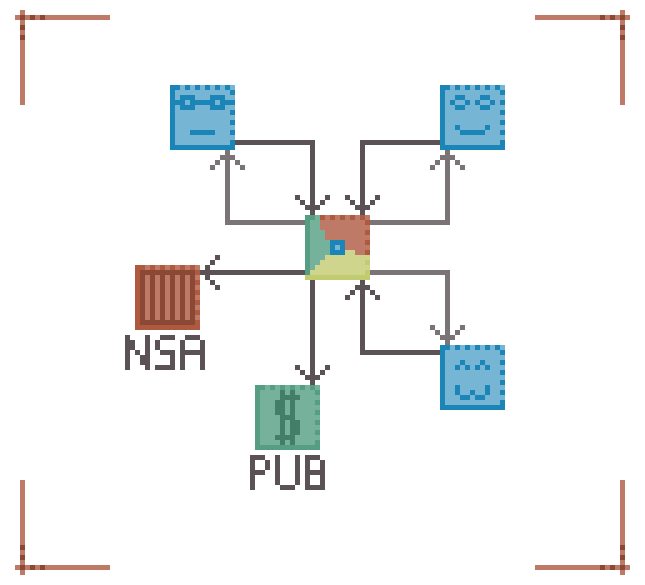
\includegraphics[width=0.95\textwidth]{img/centralizedethicproblems.png}};
      \end{tikzpicture}
    \end{center}
  \end{minipage}
  \begin{minipage}{0.32\textwidth}
    \begin{center}
      \begin{tikzpicture}
        \node[visible on=<2-3>]
        {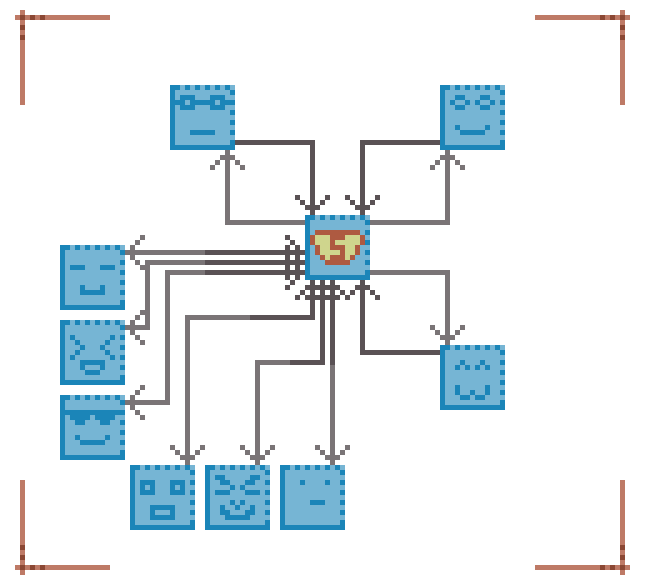
\includegraphics[width=0.95\textwidth]{img/centralizedcpuproblems.png}};
      \end{tikzpicture}
    \end{center}
  \end{minipage}
  \begin{minipage}{0.32\textwidth}
    \begin{center}
      \begin{tikzpicture}
        \node[visible on=<3-3>]
        {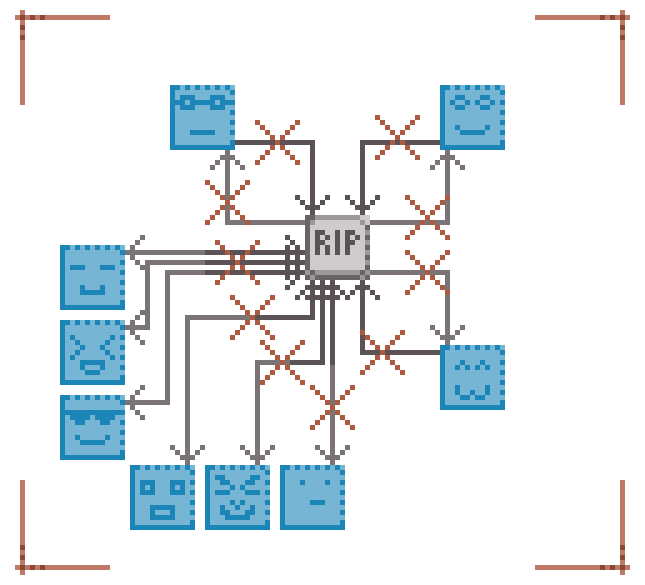
\includegraphics[width=0.95\textwidth]{img/centralizedscalabilityproblems.png}};
      \end{tikzpicture}        
    \end{center}
  \end{minipage}
\end{frame}

\begin{frame}
  En \textbf{décentralisé}, la diffusion épidémique de messages constitue une
  manière efficace de disséminer l'information.
    
  \begin{itemize}
  \item [$\rightarrow$] Rendu possible grâce à la récente technologie WebRTC :
    un navigateur peut devenir à la fois client et serveur.
    \begin{itemize}
    \item Les nœuds n'ont \textbf{ni adresses ni routes}, les connexions sont
      plus \textbf{coûteuses} et sujettes aux \textbf{defaillances} que sur
      réseau IP;
    \item Les navigateurs Web fonctionnent sur des outils aux \textbf{capacités
        hétérogènes et parfois limités};
    \item Web expose aux \textbf{pics soudains de popularité.}
    \end{itemize}
  \end{itemize}
  

\end{frame}

